% --------------------------------------------------------------
% 
% Should be compiled by XeLatex
% 
% --------------------------------------------------------------
 
\documentclass[12pt]{article}
 \usepackage[noindent]{ctex}
\usepackage{xeCJK}
\usepackage[margin=1in]{geometry} 
\usepackage{amsmath,amsthm,amssymb}
\usepackage[margin=1in]{geometry} 
\usepackage{amsmath,amsthm,amssymb}
\usepackage[english]{babel} %Castellanización
%\usepackage[T1]{fontenc} %escribe lo del teclado
\usepackage[utf8]{inputenc} %Reconoce algunos símbolos
\usepackage{lmodern} %optimiza algunas fuentes
\usepackage{graphicx}
\graphicspath{ {images/} }
\usepackage{hyperref} % Uso de links
\usepackage{url}

 
\newcommand{\N}{\mathbb{N}}
\newcommand{\Z}{\mathbb{Z}}
 
 \if0
\newenvironment{theorem}[2][Theorem]{\begin{trivlist}
\item[\hskip \labelsep {\bfseries #1}\hskip \labelsep {\bfseries #2.}]}{\end{trivlist}}
\newenvironment{lemma}[2][Lemma]{\begin{trivlist}
\item[\hskip \labelsep {\bfseries #1}\hskip \labelsep {\bfseries #2.}]}{\end{trivlist}}
\newenvironment{exercise}[2][Exercise]{\begin{trivlist}
\item[\hskip \labelsep {\bfseries #1}\hskip \labelsep {\bfseries #2.}]}{\end{trivlist}}
\newenvironment{problem}[2][Problem]{\begin{trivlist}
\item[\hskip \labelsep {\bfseries #1}\hskip \labelsep {\bfseries #2.}]}{\end{trivlist}}
\newenvironment{question}[2][Question]{\begin{trivlist}
\item[\hskip \labelsep {\bfseries #1}\hskip \labelsep {\bfseries #2.}]}{\end{trivlist}}
\newenvironment{corollary}[2][Corollary]{\begin{trivlist}
\item[\hskip \labelsep {\bfseries #1}\hskip \labelsep {\bfseries #2.}]}{\end{trivlist}}
\fi

\newenvironment{solution}{\begin{proof}[Solution]}{\end{proof}}
 
\begin{document}
 
% --------------------------------------------------------------
%                         Should be compiled by XeLatex
% --------------------------------------------------------------
 
\title{\textbf{Homework 3: Recurrent Neural Networks}}
\author{Student Name: \hspace{2in} Student ID:\\ Sun Yat-sen University}

\date{}
\maketitle
%\small
\section{\begingroup \large Exercise 1: Backpropagation through Time \endgroup}
\noindent Consider the RNN (Recurrent Neural Network) in Figure~\ref{fig:rnn}:
\begin{figure*}[h]
\label{fig:rnn}
\centering
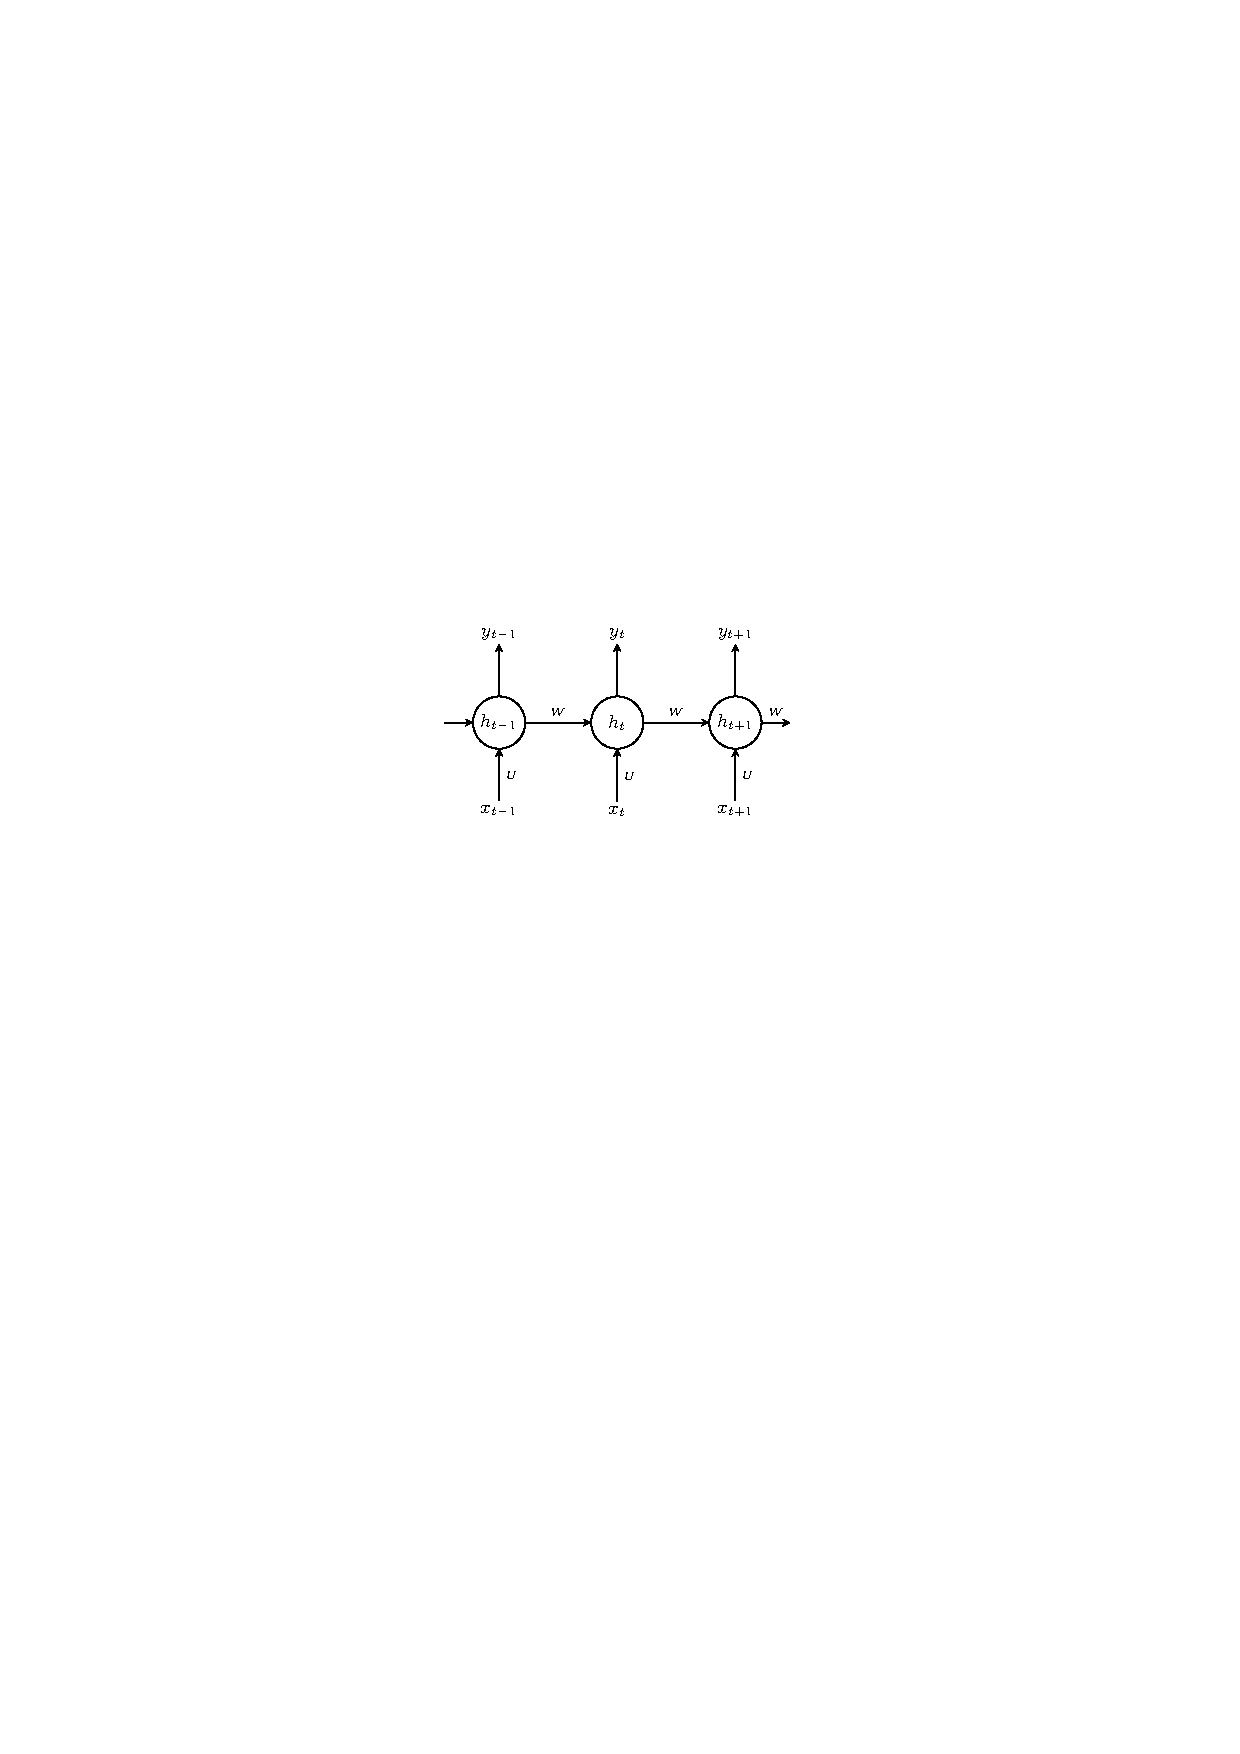
\includegraphics[scale=1.2]{rnn.pdf}
\vspace{-1em}
\caption{A recurrent neural network.}
\end{figure*}

\noindent Each state $h_t$ is given by:
\begin{equation*}
h_t = \sigma(W h_{t-1} + U x_t), \text{where } \sigma(z) =\frac{1}{1+\exp(-z)} \,.
\end{equation*}
Let $L$ be a loss function defined as the sum over the losses $L_t$ at every time step until time $T$: $L=\sum_{t=0}^T L_t$, where $L_t$ is a scalar loss depending on $h_t$.

In the following, we want to derive the gradient of this loss function with respect to the parameter $W$.

(a) Suppose we have $y=\sigma(Wx)$ where $y\in \mathbb{R}^n, x\in \mathbb{R}^d$ and $W \in \mathbb{R}^{n \times d}$. Derive the Jacobian $\frac{\partial y}{\partial x} = \mathrm{diag}(\sigma') W \in \mathbb{R}^{n \times d}$.

(b) Derive the quantity $\frac{\partial L}{\partial W} = \sum_{t=0}^T \sum_{k=1}^t \frac{\partial L_t}{\partial h_t} \frac{\partial h_t}{\partial h_k} \frac{\partial h_k}{\partial W}$. 

\section{\begingroup \large Exercise 2: Vanishing/Exploding Gradients in RNNs \endgroup}

\noindent In this exercise, we want to understand why RNNs (Recurrent Neural Networks) are especially prone to the Vanishing/Exploding Gradients problem and what role the eigenvalues of the weight matrix play. Consider part (b) of exercise 1 again.

(a) Write down $\frac{\partial L}{\partial W}$ as expanded sum for $T = 3$. You should see that if we want to backpropagate through $n$ timesteps, we have to multiply the matrix $\mathrm{diag}(\sigma')W$ $n$ times with itself.

(b) Remember that any diagonalizable (square) matrix $M$ can be represented by its eigendecomposition $M=Q\Lambda Q^{-1}$  where $Q$ is a matrix whose $i$-th column corresponds to the $i$-th eigenvector of $M$ and $\Lambda$ is a diagonal matrix with the corresponding eigenvalues placed on the diagonals. Recall that every eigenvector $v_i$ satisfies this linear equation $M v_i = \lambda_i v_i$, where $\lambda_i = \Lambda_{ii}$ is an eigenvalue of $M$. Proof by induction that for such a matrix the product $\prod_{i=1}^n M$ can be represented as: $M^n = Q \Lambda^n Q^{-1}$.

(c) Consider the weight matrix $\begin{bmatrix} 0.58 & 0.24 \\ 0.24 & 0.72 \end{bmatrix}$. Its eigendecomposition is:
\begin{equation*}
W = Q \Lambda Q^{-1} = \begin{bmatrix} 0.8 & -0.6 \\ 0.6 & 0.8 \end{bmatrix} \begin{bmatrix} 0.4 & 0 \\ 0 & 0.9 \end{bmatrix} \begin{bmatrix} 0.8 & 0.6 \\ -0.6 & 0.8 \end{bmatrix}
\end{equation*}
Calculate $W^{30}$. What do you observe? What happens in general if the absolute value of all eigenvalues of $W$ is smaller than $1$? What happens if the absolute value of any eigenvalue of $W$ is larger than $1$? What if all eigenvalues are $1$?

\section{\begingroup \large Exercise 3: LSTMs \endgroup}
 
 \noindent Recall the elements of a module in an LSTM and the corresponding computations, where $\odot$ stands for pointwise multiplication. For a good explanation on LSTMs you can refer to \url{http://colah.github.io/posts/2015-08-Understanding-LSTMs/}. Consider the LSTM in Figure~2.
 \begin{figure*}[!t]
\label{fig:lstms}
\centering
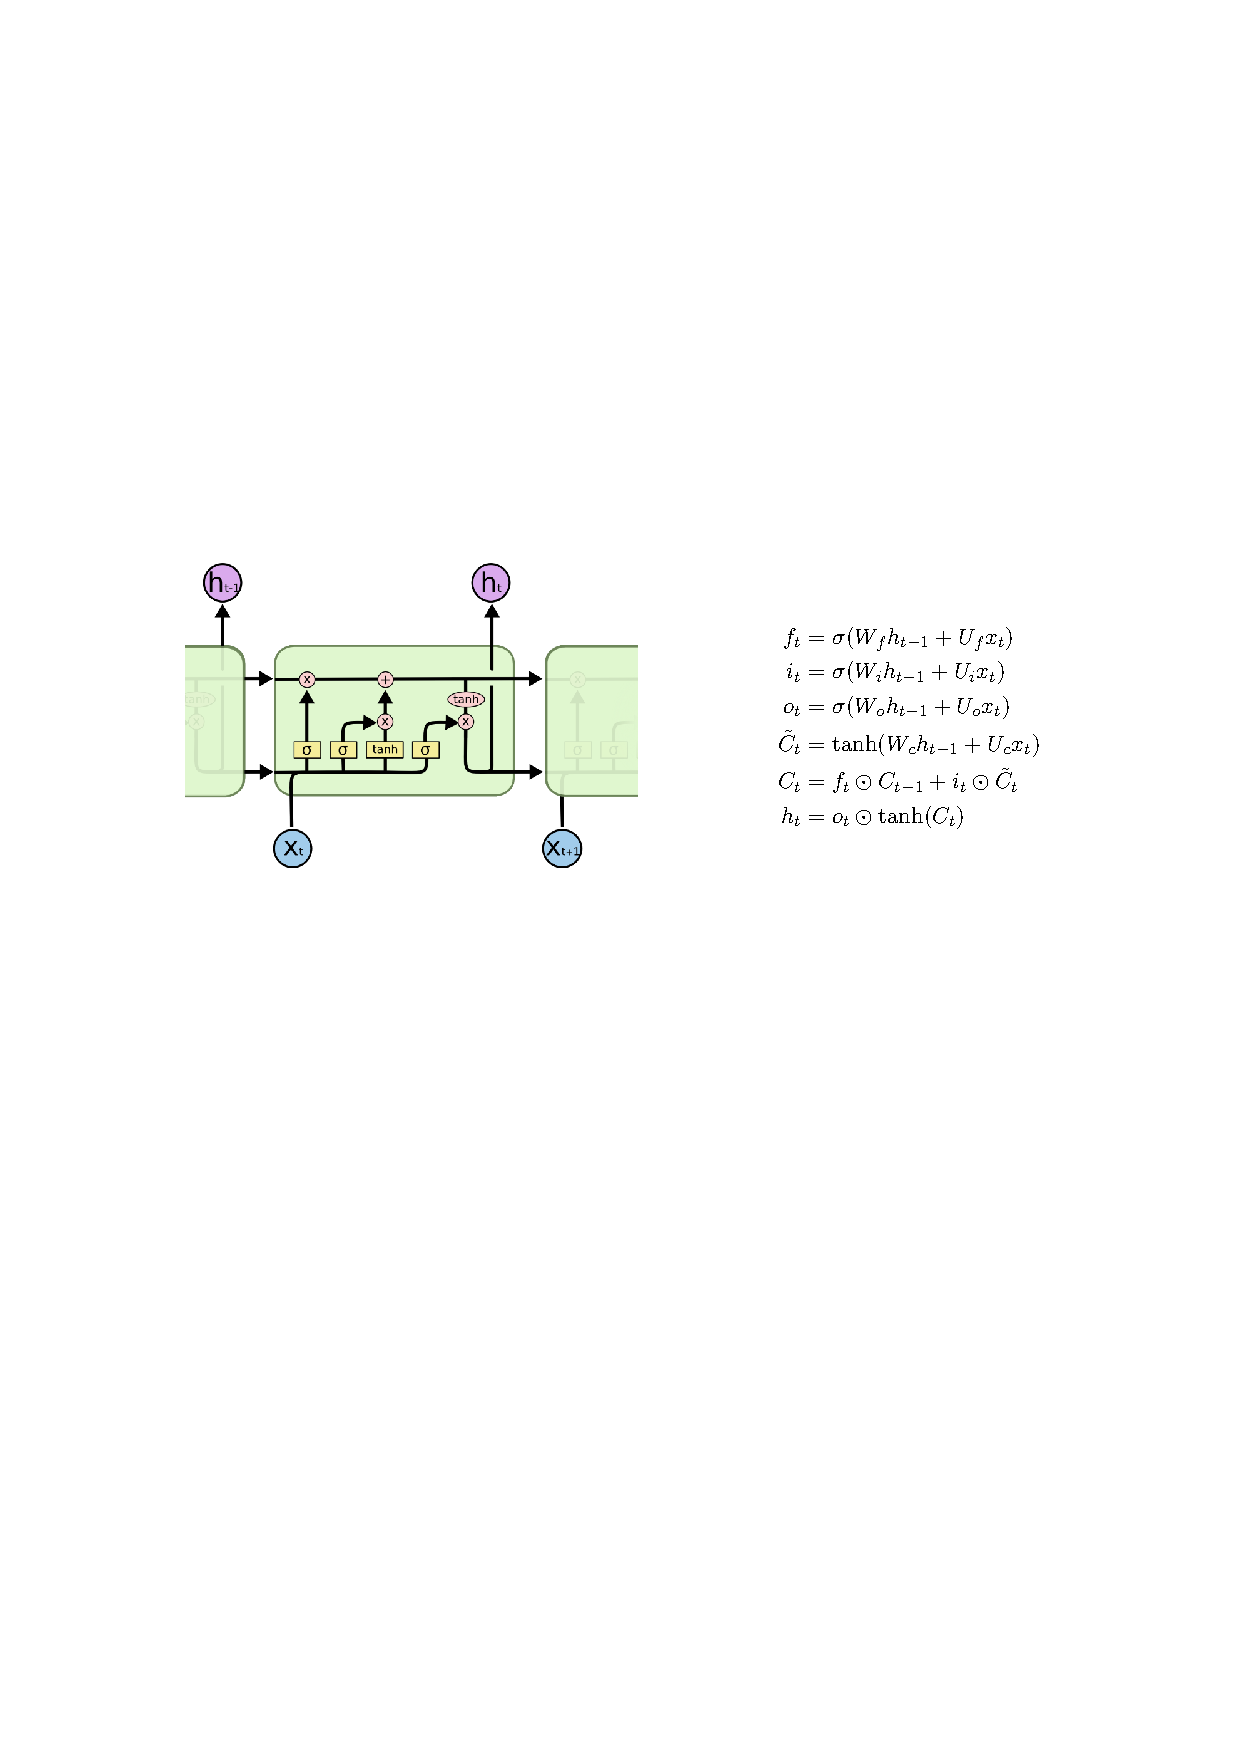
\includegraphics[scale=1.0]{lstm}
\vspace{-1em}
\caption{A Long Short Term Memory network.}
\end{figure*}
 
 (a) What do the gates $f_t$, $i_t$ and $o_t$ do?
 
 (b) Which of the quantities next to the figure are always positive?
 
 \noindent Let’s now try to understand how this architecture approaches the vanishing gradients problem. To calculate the gradient $\frac{\partial L}{\partial \theta}$, where $\theta$ stands for the parameters $(W_f, W_o, W_i, W_c)$, we now have to consider the cell state $C_t$ instead of $h_t$. Like $h_t$ in normal RNNs, $C_t$ will also depend on the previous cell states $C_{t-1}, \ldots, C_0$, so we get a formula of the form:
 \begin{equation*}
 \frac{\partial L}{\partial W} = \sum_{t=0}^T \sum_{k=1}^t \frac{\partial L}{\partial C_t} \frac{\partial C_t}{\partial C_k} \frac{\partial C_k}{\partial W},
 \end{equation*}
 where note that the real formula is a bit more complicated since $C_t$ also depends on $f_t$, $i_t$ and $\widetilde{C}_t$, which in turn all depend on $W$, but this can be neglected.
 
 (c) We know that $\frac{\partial C_t}{\partial C_k} = \prod_{i=k+1}^t \frac{\partial C_t}{\partial C_{t-1}}$. Let $f_t=1$ and $i_t=0$ such that $C_t = C_{t-1}$ for all $t$. What is the gradient $\frac{\partial C_t}{\partial C_k}$ in this case?
 
 
 
\end{document}